% \documentclass[table]{beamer}
\documentclass[table,handout]{beamer}
\setbeameroption{show notes}
% \setbeameroption{hide notes}
% \setbeameroption{show only notes}
\usepackage{varwidth}

\newif\ifhide
\newif\ifpost
\newif\ifhideclicker

% \hidetrue
% \hideclickertrue
% \posttrue

\newcommand{\whiteout}[1]{\textcolor{white}{#1}}
% \newcommand{\whiteoutbox}[1]{\fcolorbox{white}{white}{\parbox{\dimexpr \linewidth-2\fboxsep-2\fboxrule}{\whiteout{#1}}}}
% \newcommand{\notebox}[1]{\fcolorbox{blue}{white}{\parbox{\dimexpr \linewidth-2\fboxsep-2\fboxrule}{#1}}}
\newcommand{\whiteoutbox}[1]{\fcolorbox{white}{white}{\parbox{\linewidth}{\whiteout{#1}}}}
\newcommand{\notebox}[1]{\fcolorbox{blue}{white}{\parbox{\linewidth}{#1}}}
\newcommand{\blankbox}[1]{\phantom{\varwidth{\linewidth}\whiteoutbox{#1}\endvarwidth}}
\newcommand{\blank}[1]{\phantom{\varwidth{\linewidth}#1\endvarwidth}}

\ifhide%
    \newcommand{\hmask}[1]{\blank{#1}}%
\else%
    \newcommand{\hmask}[1]{#1}%
\fi

\ifhide%
    \newcommand{\wout}[1]{\whiteout{#1}}%
\else%
    \newcommand{\wout}[1]{#1}%
\fi

\ifhide%
    \newcommand{\hignore}[1]{}%
\else%
    \newcommand{\hignore}[1]{#1}%
\fi

\ifpost%
    \newcommand{\nopost}[1]{}%
\else%
    \newcommand{\nopost}[1]{#1}%
\fi

\ifhideclicker%
    \newcommand{\clickerslide}[1]{\stepcounter{clickerQuestionCounter}%
        \begin{frame}[t]
            \textcolor{blue}{Q \arabic{clickerQuestionCounter}:}
        \end{frame}}
\else%
    \newcommand{\clickerslide}[1]{#1}%
\fi

\ifhide%
    \newcommand{\hidebox}[1]{\blank{#1}}%
\else%
    \newcommand{\hidebox}[1]{\notebox{#1}}%
\fi

\ifhide%
    \newcommand{\wbox}[1]{\whiteoutbox{#1}}%
\else%
    \newcommand{\wbox}[1]{\notebox{#1}}%
\fi

\ifhide%
    \newcommand{\nbox}[1]{\blankbox{#1}}%
\else%
    \newcommand{\nbox}[1]{\notebox{#1}}%
\fi

\ifhideclicker%
    \newcommand{\clickeranswer}[1]{#1}%
\else%
    \ifhide%
        \newcommand{\clickeranswer}[1]{#1}%
    \else%
        \newcommand{\clickeranswer}[1]{\textbf{\textcolor{blue}{#1}}}%
    \fi
\fi

\usepackage{beamerthemesplit}
% \usetheme{boxes}
\usetheme{Malmoe}
\usecolortheme{seahorse}
% \usecolortheme{seagull}
\usepackage{ifthen}
\usepackage{xspace}
\usepackage{multirow}
\usepackage{multicol}
\usepackage{booktabs}
\usepackage{xcolor}
\usepackage{wasysym}
\usepackage{comment}
\usepackage{hyperref}
\hypersetup{pdfborder={0 0 0}, colorlinks=true, urlcolor=blue, linkcolor=blue, citecolor=blue}
\usepackage{changepage}
\usepackage[compatibility=false]{caption}
\captionsetup[figure]{font=scriptsize, labelformat=empty, textformat=simple, justification=centering, skip=2pt}
\usepackage{tikz}
\usetikzlibrary{trees,calc,backgrounds}

\usepackage[bibstyle=joaks-slides,maxcitenames=3,mincitenames=1,backend=biber]{biblatex}

\newrobustcmd*{\shortfullcite}{\AtNextCite{\renewbibmacro{title}{}\renewbibmacro{in:}{}\renewbibmacro{number}{}}\fullcite}

\newrobustcmd*{\footlessfullcite}{\AtNextCite{\renewbibmacro{title}{}\renewbibmacro{in:}{}}\footfullcite}

% Make all footnotes smaller
% \renewcommand{\footnotesize}{\scriptsize}

\definecolor{myGray}{gray}{0.9}
\colorlet{rowred}{red!30!white}

\setbeamertemplate{blocks}[rounded][shadow=true]

\setbeamercolor{defaultcolor}{bg=structure!30!normal text.bg,fg=black}
\setbeamercolor{block body}{bg=structure!30!normal text.bg,fg=black}
\setbeamercolor{block title}{bg=structure!50!normal text.bg,fg=black}

\newenvironment<>{varblock}[2][\textwidth]{%
  \setlength{\textwidth}{#1}
  \begin{actionenv}#3%
    \def\insertblocktitle{#2}%
    \par%
    \usebeamertemplate{block begin}}
  {\par%
    \usebeamertemplate{block end}%
  \end{actionenv}}

\newenvironment{displaybox}[1][\textwidth]
{
    \centerline\bgroup\hfill
    \begin{beamerboxesrounded}[lower=defaultcolor,shadow=true,width=#1]{}
}
{
    \end{beamerboxesrounded}\hfill\egroup
}

\newenvironment{onlinebox}[1][4cm]
{
    \newbox\mybox
    \newdimen\myboxht
    \setbox\mybox\hbox\bgroup%
        \begin{beamerboxesrounded}[lower=defaultcolor,shadow=true,width=#1]{}
    \centering
}
{
    \end{beamerboxesrounded}\egroup
    \myboxht\ht\mybox
    \raisebox{-0.25\myboxht}{\usebox\mybox}\hspace{2pt}
}

\newenvironment{mydescription}{
    \begin{description}
        \setlength{\leftskip}{-1.5cm}}
    {\end{description}}

\newenvironment{myitemize}{
    \begin{itemize}
        \setlength{\leftskip}{-.3cm}}
    {\end{itemize}}

% footnote without a marker
\newcommand\barefootnote[1]{%
  \begingroup
  \renewcommand\thefootnote{}\footnote{#1}%
  \addtocounter{footnote}{-1}%
  \endgroup
}

% define formatting for footer
\newcommand{\myfootline}{%
    {\it
    \insertshorttitle
    \hspace*{\fill} 
    \insertshortauthor, \insertshortinstitute
    % \ifx\insertsubtitle\@empty\else, \insertshortsubtitle\fi
    \hspace*{\fill}
    \insertframenumber/\inserttotalframenumber}}

% set up footer
\setbeamertemplate{footline}{%
    \usebeamerfont{structure}
    \begin{beamercolorbox}[wd=\paperwidth,ht=2.25ex,dp=1ex]{frametitle}%
        % \Tiny\hspace*{4mm}\myfootline\hspace{4mm}
        \tiny\hspace*{4mm}\myfootline\hspace{4mm}
    \end{beamercolorbox}}

% remove navigation bar
\beamertemplatenavigationsymbolsempty

\makeatletter
    \newenvironment{noheadline}{
        \setbeamertemplate{headline}[default]
        \def\beamer@entrycode{\vspace*{-\headheight}}
    }{}
\makeatother

\newcounter{clickerQuestionCounter}
\ifhideclicker%
\newenvironment{clickerquestion}
{ \stepcounter{clickerQuestionCounter}
  \begin{enumerate}[Q \arabic{clickerQuestionCounter}:]\color{white} }
{ \end{enumerate} }
\else%
\newenvironment{clickerquestion}
{ \stepcounter{clickerQuestionCounter}
  \begin{enumerate}[Q \arabic{clickerQuestionCounter}:] }
{ \end{enumerate} }
\fi

\ifhideclicker%
\newenvironment{clickeroptions}
{ \begin{enumerate}[\begingroup\color{white} 1)\endgroup]\color{white} }
{ \end{enumerate} }
\else%
\newenvironment{clickeroptions}
{ \begin{enumerate}[\begingroup\color{red} 1)\endgroup] }
{ \end{enumerate} }
\fi


\tikzstyle{centered} = [align=center, text centered, font=\sffamily\bfseries]
\tikzstyle{skip} = [centered, inner sep=0pt, fill]
\tikzstyle{empty} = [centered, inner sep=0pt]
\tikzstyle{inode} = [centered, circle, minimum width=4pt, fill=black, inner sep=0pt]
\tikzstyle{tnode} = [centered, circle, inner sep=1pt]
\tikzset{
  % edge styles
  level distance=10mm,
  mate/.style={edge from parent/.style={draw,distance=3pt}},
  mleft/.style={grow=left, level distance=10mm, edge from parent path={(\tikzparentnode.west)--(\tikzchildnode.east)}},
  mright/.style={grow=right, level distance=10mm, edge from parent path={(\tikzparentnode.east)--(\tikzchildnode.west)}},
  % node styles
  male/.style={rectangle,minimum size=4mm,fill=gray!80},
  female/.style={circle,minimum size=4mm,fill=gray!80},
  amale/.style={male,fill=red},
  afemale/.style={female,fill=red},
}

\newcommand{\highlight}[1]{\textcolor{violet}{\textit{\textbf{#1}}}}
\newcommand{\super}[1]{\ensuremath{^{\textrm{\sffamily #1}}}}
\newcommand{\sub}[1]{\ensuremath{_{\textrm{\sffamily #1}}}}
\newcommand{\dC}{\ensuremath{^\circ{\textrm{C}}}}
\newcommand{\tb}{\hspace{2em}}
\providecommand{\e}[1]{\ensuremath{\times 10^{#1}}}
\newcommand{\myHangIndent}{\hangindent=5mm}

\newcommand{\spp}[1]{\textit{#1}}

\newcommand\mybullet{\leavevmode%
\usebeamertemplate{itemize item}\hspace{.5em}}

\makeatletter
\newcommand*{\rom}[1]{\expandafter\@slowromancap\romannumeral #1@}
\makeatother

\newcommand{\blankslide}{{\setbeamercolor{background canvas}{bg=black}
\setbeamercolor{whitetext}{fg=white}
\begin{frame}<handout:0>[plain]
\end{frame}}}

\newcommand{\whiteslide}{
\begin{frame}<handout:0>[plain]
\end{frame}}

\newcommand{\f}[1]{\ensuremath{F_{#1}}}
\newcommand{\x}[1]{X\ensuremath{^{#1}}}
\newcommand{\y}[1]{Y\ensuremath{^{#1}}}

% Population growth macros
\newcommand{\popsize}[1]{\ensuremath{N_{#1}}}
\newcommand{\popgrowthratediscrete}[1]{\ensuremath{\lambda_{#1}}}
\newcommand{\popgrowthrate}[1]{\ensuremath{r_{#1}}}
\newcommand{\ptime}{\ensuremath{t}\xspace}

\tikzset{hide on/.code={\only<#1>{\color{white}}}}
\tikzset{
    invisible/.style={opacity=0},
    visible on/.style={alt={#1{}{invisible}}},
    alt/.code args={<#1>#2#3}{%
        \alt<#1>{\pgfkeysalso{#2}}{\pgfkeysalso{#3}}
        % \pgfkeysalso doesn't change the path
    },
}

\bibliography{../bib/references}
\author[J.\ Oaks]{
    %Jamie R.\ Oaks\inst{1}
    Jamie R.\ Oaks
}
\institute[BIOL 180]{
    \inst{}%
        BIOL 180: Introductory Biology
}



\title{Ecosystems II}
\subtitle{Climate Change}
% \date{\today}
\date{June 2, 2015}

% \setbeamertemplate{section in toc}[sections numbered]
% \setbeamertemplate{subsection in toc}[subsections numbered]

\begin{document}

\begin{noheadline}
\maketitle
\end{noheadline}

\nopost{
\begin{noheadline}
\begin{frame}[c]
    \vspace{-6mm}
    \begin{center} 
        \includegraphics[height=1.2\textheight]{../images/seating-chart-2.pdf}
    \end{center}
\end{frame}
\end{noheadline}
}

\clickerslide{
\begin{noheadline}
\begin{frame}
    \begin{clickerquestion}
        \item When ecologist friends of mine are asked why they are vegetarian,
            they often reply, ``It's more efficient.'' What do they mean?
 
        \begin{clickeroptions}
            \item It's a faster, safer, and more-effective way to lose weight
                than high-protein (high meat) diets.
            \item \clickeranswer{Eating primary producers instead of consumers
                    avoids energy losses.}
            \item He is diversifying his sources of protein and fat instead of
                relying primarily on animal sources.
            \item It’s cheaper (meat costs more than grains, beans, and
                vegetables).
        \end{clickeroptions}
    \end{clickerquestion}
\end{frame}
\end{noheadline}
}

% \clickerslide{
% \begin{noheadline}
% \begin{frame}
%     \begin{clickerquestion}
%         \item As Chinese people have become wealthier, demand for meat has
%             increased dramatically. What is the most likely consequence?
%  
%         \begin{clickeroptions}
%             \item Population growth rate will slow.
%             \item \clickeranswer{China may have to start importing grain
%                     again.}
%             \item Economic growth will increase even more.
%             \item The sex ratio may become imbalanced, in favor of males.
%         \end{clickeroptions}
%     \end{clickerquestion}
% \end{frame}
% \end{noheadline}
% }

\begin{noheadline}
\begin{frame}
\frametitle{Today's issues:}
% \tableofcontents[subsectionstyle=hide]
\tableofcontents
\end{frame}
\end{noheadline}

\section{I. How are humans changing the carbon cycle?}

\subsection{A. What is the carbon cycle in terrestrial ecosystems?}

\begin{frame}
    A. What is the carbon cycle in terrestrial ecosystems?\\

    \vspace{0.5cm}
    \begin{tikzpicture}[>=latex]%,xscale=0.3,yscale=0.3]
    
        % Styles for reservoirs, and reservoir edges
        \tikzstyle{state} = [draw, fill=structure!20!, rectangle,
            minimum height=2em,
            minimum width=4em,
            node distance=4em,
            font={\sffamily\bfseries}]
        \tikzstyle{stateEdgePortion} = [black,ultra thick];
        \tikzstyle{stateEdge} = [stateEdgePortion,->];
        \tikzstyle{edgeLabel} = [pos=0.5, text centered, font={\sffamily\small}];
    
        % Reservoirs
        \node[state, name=atmosphere] {CO\sub{2} in Atmosphere};
        \node[state, name=primaryproducers, below of=atmosphere] {Primary producers};
        \node[state, name=consumerweb,
            below of=primaryproducers,
            left of=primaryproducers,
            xshift=-4em
            ] {\ Consumer food web\ \ };
        \node[state, name=decomposerweb,
            below of=primaryproducers,
            right of=primaryproducers,
            xshift=4em
            ] {Decomposer food web};
        \node[state, name=sinks, below of=decomposerweb] {Humus (SOM), peat, coal};
    
        % Connect States via edges
        \begin{uncoverenv}<0|handout:1>
        \draw ($(atmosphere.south)
                + (-.5em,0)
            $) 
            edge[stateEdge] node[edgeLabel,
                % xshift=-3em
            ]{} 
            ($(primaryproducers.north)
                + (-.5em,0)
            $); 
        \draw ($(primaryproducers.north)
                + (.5em,0)
            $) 
            edge[stateEdge] node[edgeLabel,
                % xshift=2em
            ]{} 
            ($(atmosphere.south)
                + (.5em,0)
            $);
    
        \draw ($(primaryproducers.south)
                + (-.5em,0)
            $) 
            edge[stateEdge, bend left=22.5] node[edgeLabel,
                % xshift=-2em,
                % yshift=1em
                ]{} 
            ($(consumerweb.east)
                + (0,.5em)
            $);
        \draw ($(primaryproducers.south)
                + (.5em,0)
            $) 
            edge[stateEdge, bend right=22.5] node[edgeLabel,
                % xshift=1em,
                % yshift=1em
                ]{} 
            ($(decomposerweb.west)
                + (0,.5em)
            $);
    
        \draw ($(consumerweb.north)
                % + (.5em,0)
            $) 
            edge[stateEdge, bend left=45] node[edgeLabel,
                % xshift=-4em
            ]{} 
            ($(atmosphere.west)
                % + (0,-.5em)
            $);
    
        \draw ($(decomposerweb.north)
                % + (-.5em,0)
            $) 
            edge[stateEdge, bend right=45] node[edgeLabel,
                % xshift=-1em,
                % yshift=-1em
                ]{} 
            ($(atmosphere.east)
                % + (0,-.5em)
            $);
        \draw ($(consumerweb.east)$)
            edge[stateEdge] node[edgeLabel]{}
            ($(decomposerweb.west)$);
    
        \draw ($(decomposerweb.south)
                % + (-.5em,0)
            $) 
            edge[stateEdge] node[edgeLabel,
                % xshift=-3em
                ]{} 
            ($(sinks.north)
                % + (-.5em,0)
            $); 
        % \draw ($(sinks.north)
        %         + (.5em,0)
        %         $) 
        %     edge[stateEdge] node[edgeLabel,
        %         % xshift=2em
        %         ]{} 
        %     ($(decomposerweb.south)
        %         + (.5em,0)
        %         $);
        \end{uncoverenv}
    \end{tikzpicture}

    \vspace{2mm}
    What are the key carbon sinks on land? \\
    \nbox{Wood, peat, soil}

    \note[item]{Atmosphere to primary producers; portion released back as
        byproduct of respiration}
    \note[item]{PPs to consumers; portion released as byproduct of
        respiration}
    \note[item]{to decomposers (bacteria \& fungi); released via respiration}
    \note[item]{Some to terrestrial sinks: SOM, peat, coal}
\end{frame}

\subsection{B. What is the carbon cycle in marine ecosystems?}

\begin{frame}
    B. What is the carbon cycle in marine ecosystems?\\

    \vspace{0.5cm}
    \begin{tikzpicture}[>=latex]%,xscale=0.3,yscale=0.3]
    
        % Styles for reservoirs, and reservoir edges
        \tikzstyle{state} = [draw, fill=structure!20!, rectangle,
            minimum height=2em,
            minimum width=4em,
            node distance=4em,
            font={\sffamily\bfseries}]
        \tikzstyle{stateEdgePortion} = [black,ultra thick];
        \tikzstyle{stateEdge} = [stateEdgePortion,->];
        \tikzstyle{edgeLabel} = [pos=0.5, text centered, font={\sffamily\small}];
    
        % Reservoirs
        \node[state, name=atmosphere] {CO\sub{2} in Atmosphere};
        \node[state, name=primaryproducers, below of=atmosphere] {Primary producers};
        \node[state, name=consumerweb,
            below of=primaryproducers,
            left of=primaryproducers,
            xshift=-4em
            ] {\ Consumer food web\ \ };
        \node[state, name=decomposerweb,
            below of=primaryproducers,
            right of=primaryproducers,
            xshift=4em
            ] {Decomposer food web};
        \node[state, name=sinks, below of=decomposerweb,
            xshift=-7em
            ] {DOM, organics in
            benthos, limestone, shale, petroleum};

        \begin{uncoverenv}<0|handout:1>
        % Connect States via edges
        \draw ($(atmosphere.south)
                + (-.5em,0)
            $) 
            edge[stateEdge] node[edgeLabel,
                % xshift=-3em
            ]{} 
            ($(primaryproducers.north)
                + (-.5em,0)
            $); 
        \draw ($(primaryproducers.north)
                + (.5em,0)
            $) 
            edge[stateEdge] node[edgeLabel,
                % xshift=2em
            ]{} 
            ($(atmosphere.south)
                + (.5em,0)
            $);
    
        \draw ($(primaryproducers.south)
                + (-.5em,0)
            $) 
            edge[stateEdge, bend left=22.5] node[edgeLabel,
                % xshift=-2em,
                % yshift=1em
                ]{} 
            ($(consumerweb.east)
                + (0,.5em)
            $);
        \draw ($(primaryproducers.south)
                + (.5em,0)
            $) 
            edge[stateEdge, bend right=22.5] node[edgeLabel,
                % xshift=1em,
                % yshift=1em
                ]{} 
            ($(decomposerweb.west)
                + (0,.5em)
            $);
    
        \draw ($(consumerweb.north)
                % + (.5em,0)
            $) 
            edge[stateEdge, bend left=45] node[edgeLabel,
                % xshift=-4em
            ]{} 
            ($(atmosphere.west)
                % + (0,-.5em)
            $);
    
        \draw ($(decomposerweb.north)
                % + (-.5em,0)
            $) 
            edge[stateEdge, bend right=45] node[edgeLabel,
                % xshift=-1em,
                % yshift=-1em
                ]{} 
            ($(atmosphere.east)
                % + (0,-.5em)
            $);
        \draw ($(consumerweb.east)$)
            edge[stateEdge] node[edgeLabel]{}
            ($(decomposerweb.west)$);
    
        \draw ($(decomposerweb.south)
                % + (-.5em,0)
            $) 
            edge[stateEdge] node[edgeLabel,
                % xshift=-3em
                ]{} 
            ($(sinks.north)
                + (7em,0)
            $); 
        % \draw ($(sinks.north)
        %         + (.5em,0)
        %         $) 
        %     edge[stateEdge] node[edgeLabel,
        %         % xshift=2em
        %         ]{} 
        %     ($(decomposerweb.south)
        %         + (.5em,0)
        %         $);
        \end{uncoverenv}
    \end{tikzpicture}

    \vspace{2mm}
    What are the key carbon sinks in the ocean? \\
    \nbox{DOM, organic matter in benthos, limestone, shale, oil formation}
\end{frame}

\subsection{C. Human impacts on the carbon cycle}

\begin{frame}
    C. Human impacts on the carbon cycle \\

    \vspace{-7mm}
    \begin{center} 
        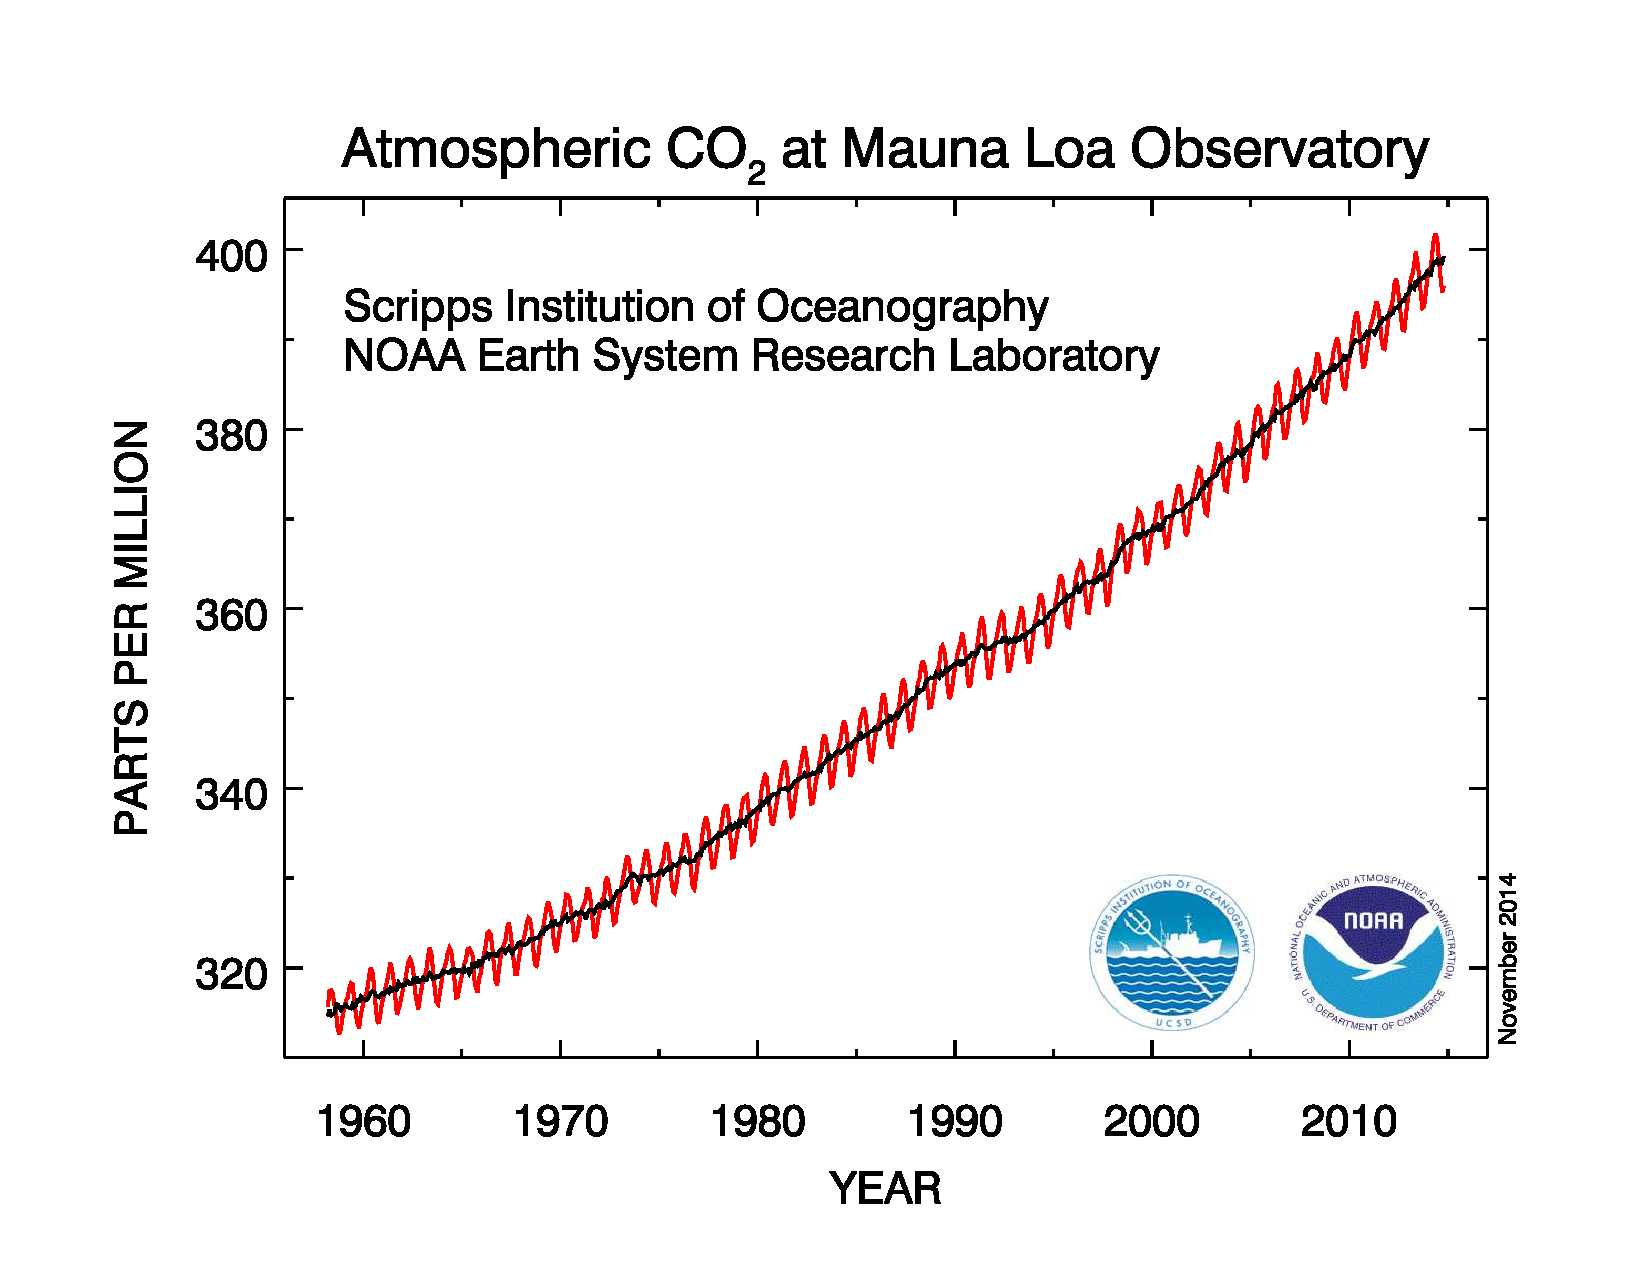
\includegraphics[width=\textwidth]{../images/co2-data-mauna-loa-observatory.pdf}
    \end{center}
    \note[item]{Why recorded in Mauna Loa (volcano), Island of Hawaii?}
    \note[item]{NOAA observatory at 3400m (11,150ft)}
\end{frame}

\begin{frame}
    C. Human impacts on the carbon cycle \\

    \vspace{-7mm}
    \begin{center} 
        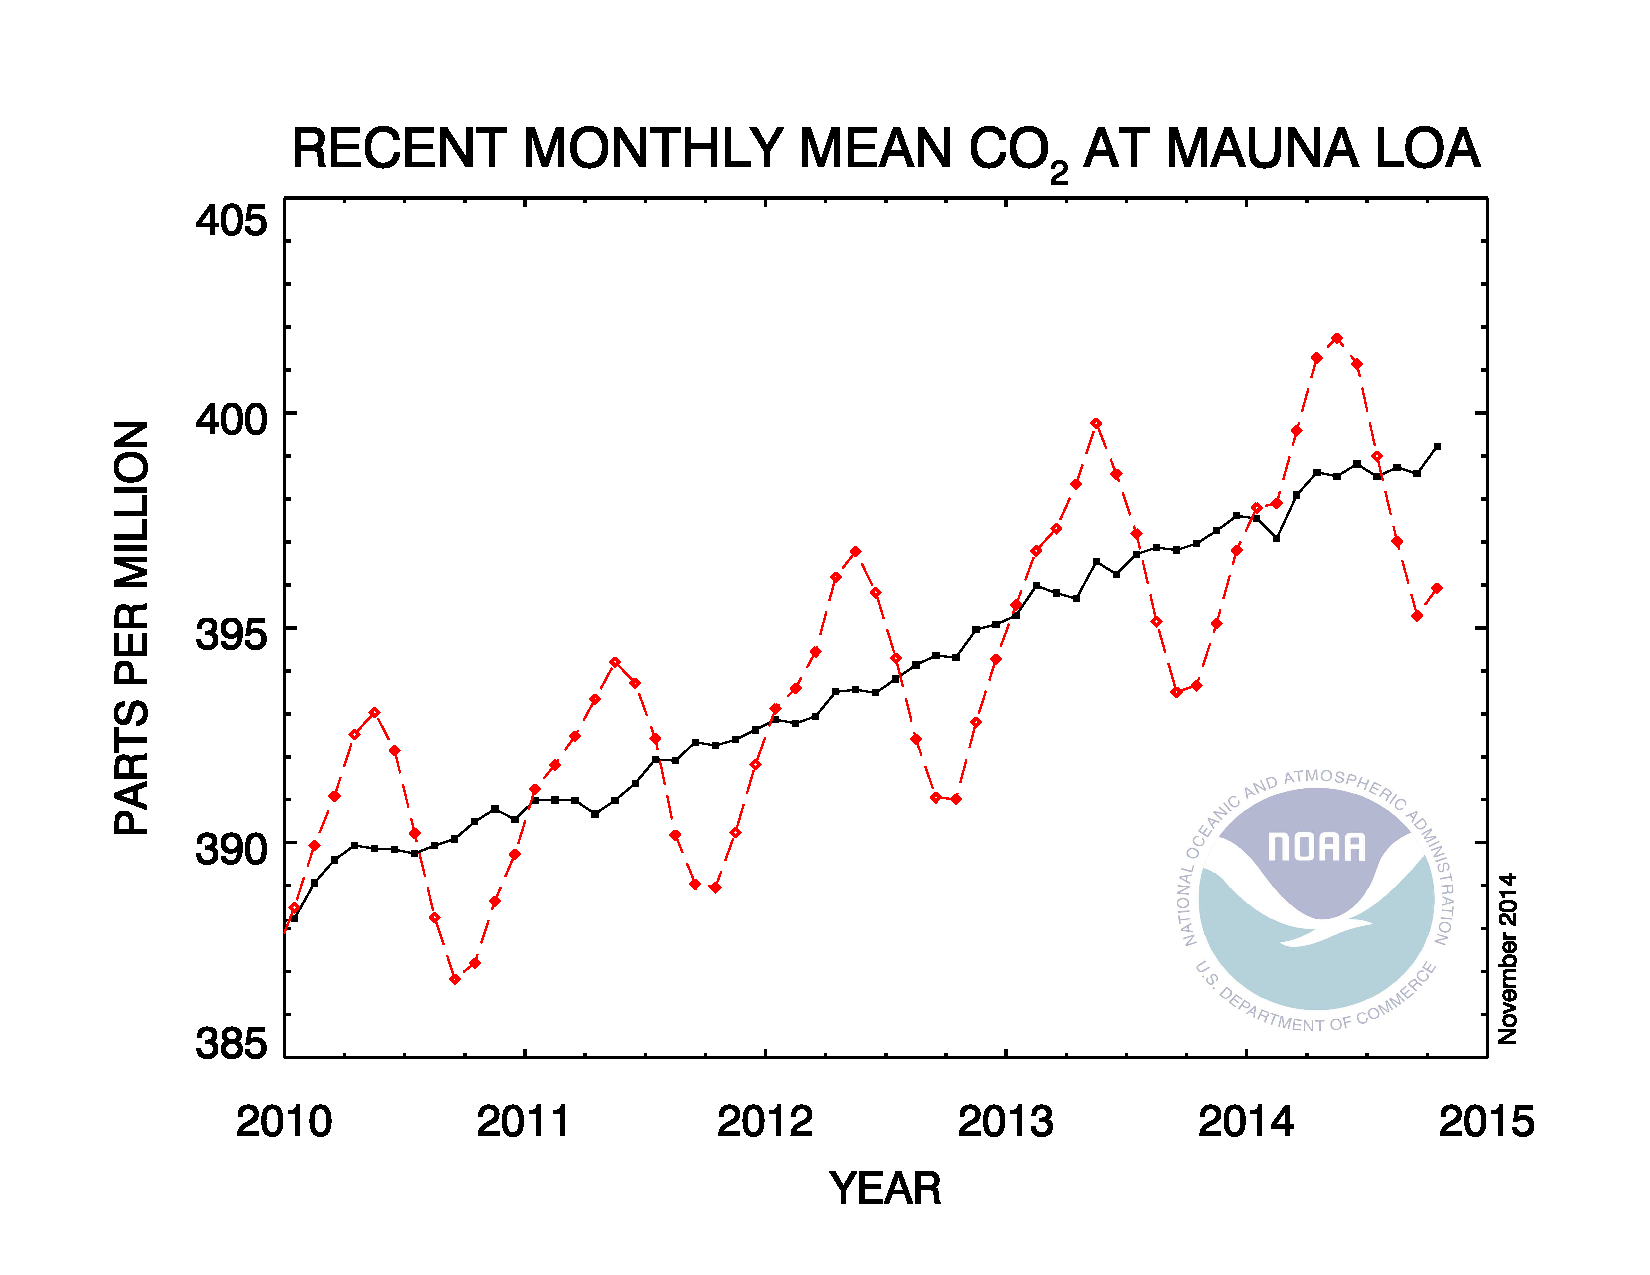
\includegraphics[width=\textwidth]{../images/co2-trend-mauna-loa-observatory.pdf}
    \end{center}
    \note[item]{Red is actual measurement (black is average over seasons); why
        the oscillations?}
\end{frame}

\clickerslide{
\begin{frame}
    \begin{adjustwidth}{-2em}{-1.5em}

    \begin{columns}

        \column{0.5\linewidth}

        \begin{clickerquestion}
            \item Why do these data ``zig-zag?''
        \end{clickerquestion}
        \begin{clickeroptions}
            \small
            \item Because there has been a dramatic increase in the
                concentration of atmospheric CO\sub{2} over time. 
            \item Because increased concentrations of CO\sub{2} are
                contributing to global warming.
            \item \clickeranswer{High points at end of winter; low points
                    at end of summer.  (Most photosynthesis occurs in the
                    northern hemisphere.)}
            \item High points are at end of summer; low points are at end
                of winter.  (Most photosynthesis occurs in the northern
                hemisphere.)
        \end{clickeroptions}

        \column{0.5\linewidth}

        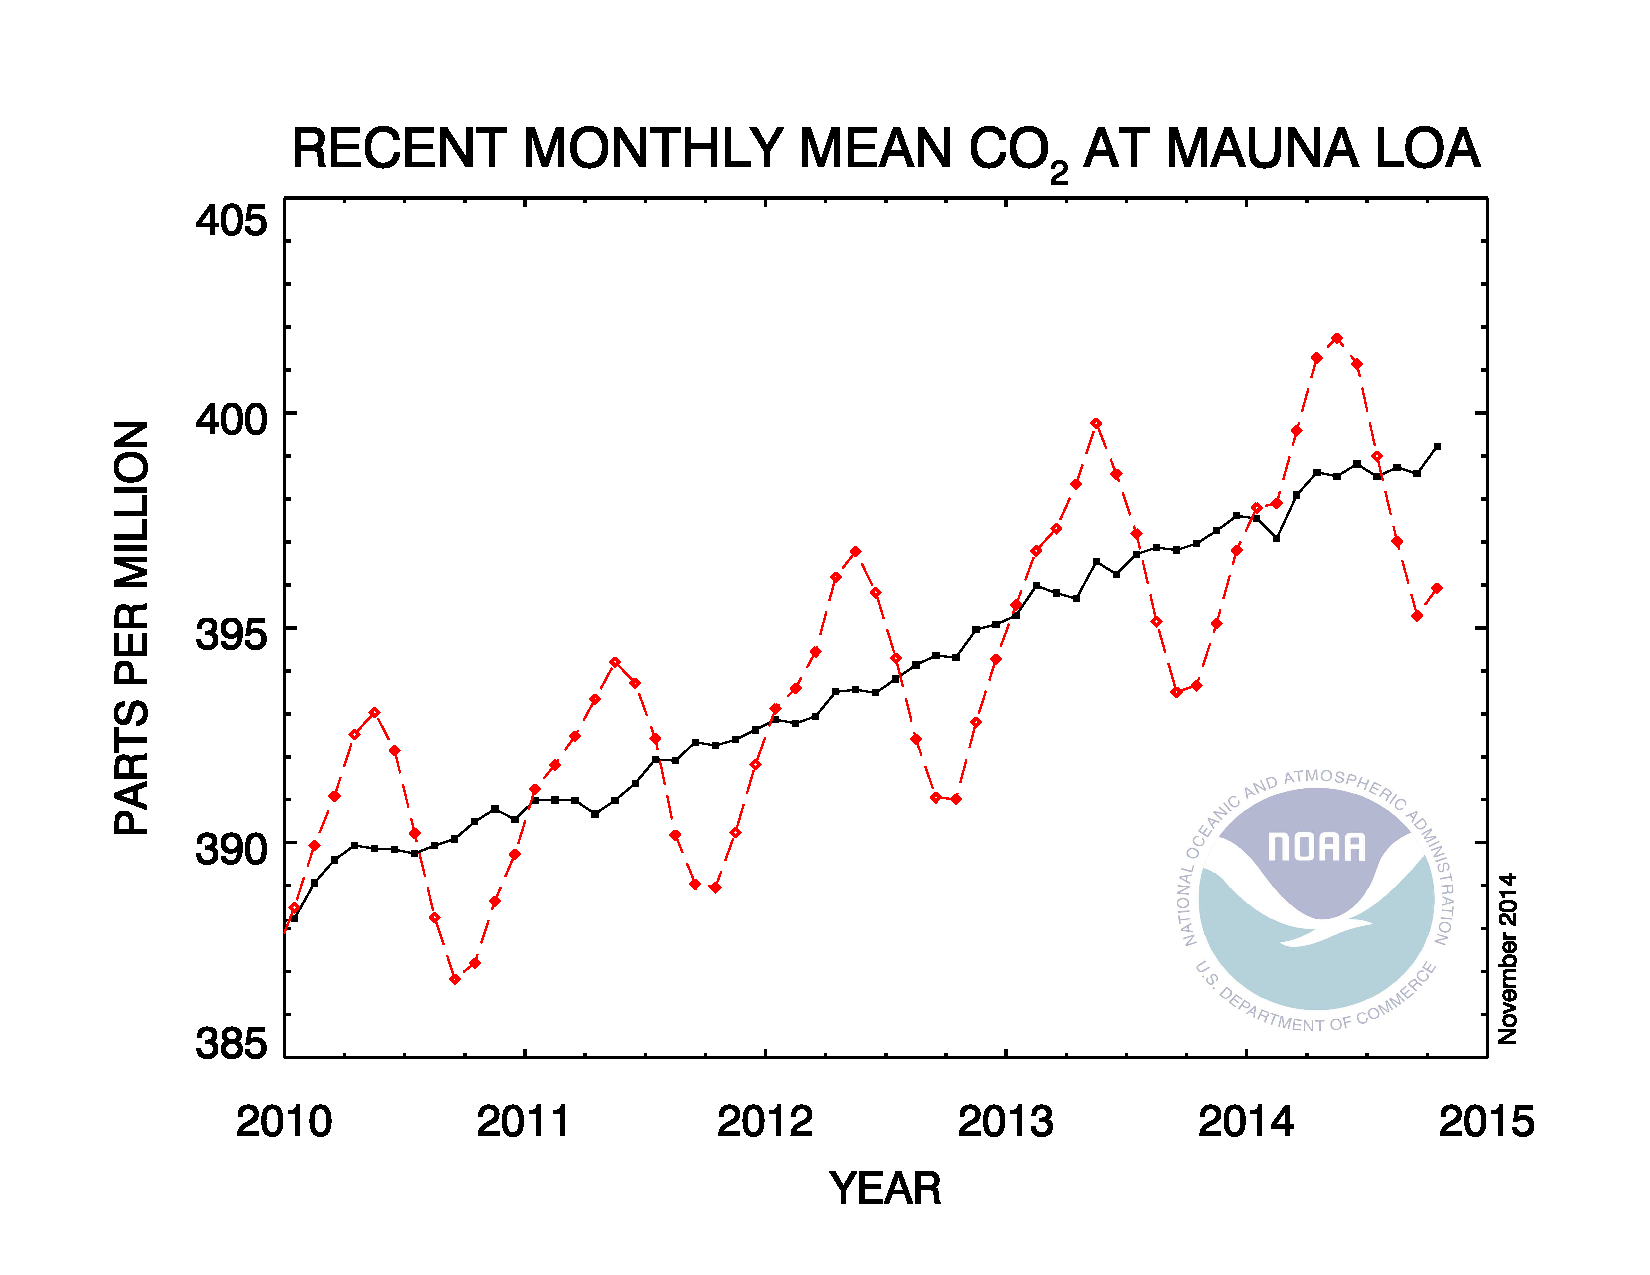
\includegraphics[width=\columnwidth]{../images/co2-trend-mauna-loa-observatory.pdf}

    \end{columns}
    \end{adjustwidth}
\end{frame}
}

\clickerslide{
\begin{frame}
    \begin{clickerquestion}
        \item Why are these data important for the climate?

        \begin{clickeroptions}
            \item CO\sub{2} absorbs high-energy solar radiation, which traps
                energy in the atmosphere, causing warming.
            \item CO\sub{2} reflects high-energy solar radiation back
                out of the atmosphere; this generates heat and
                warms the atmosphere.
            \item \clickeranswer{CO\sub{2} absorbs infrared radiation emitted
                    by the Earth's surface, trapping heat in the atmosphere.}
            \item Increased CO\sub{2} leads to increased primary productivity,
                which produces heat.
        \end{clickeroptions}
    \end{clickerquestion}
\end{frame}
}


\begin{frame}
    \begin{adjustwidth}{-2em}{-1.5em}
    \begin{columns}

        \column{0.26\linewidth}
        {\small
        How much has the average land air temperature increased since 1900?

        \nbox{\tiny land: $\approx$1\dC}
        
        \vspace{2mm}
        How does this compare to marine air temperature?

        \nbox{\tiny marine: $\approx$0.6\dC. The air above
            the ocean is insulated by the much denser water}

        \vspace{2mm}
        How much has average global sea level increased since 1900?
        
        \nbox{\scriptsize $\approx$0.2m}
        }

        \column{0.73\linewidth}
        \vspace{-0.1cm}
        \begin{figure}
        \begin{center} 
            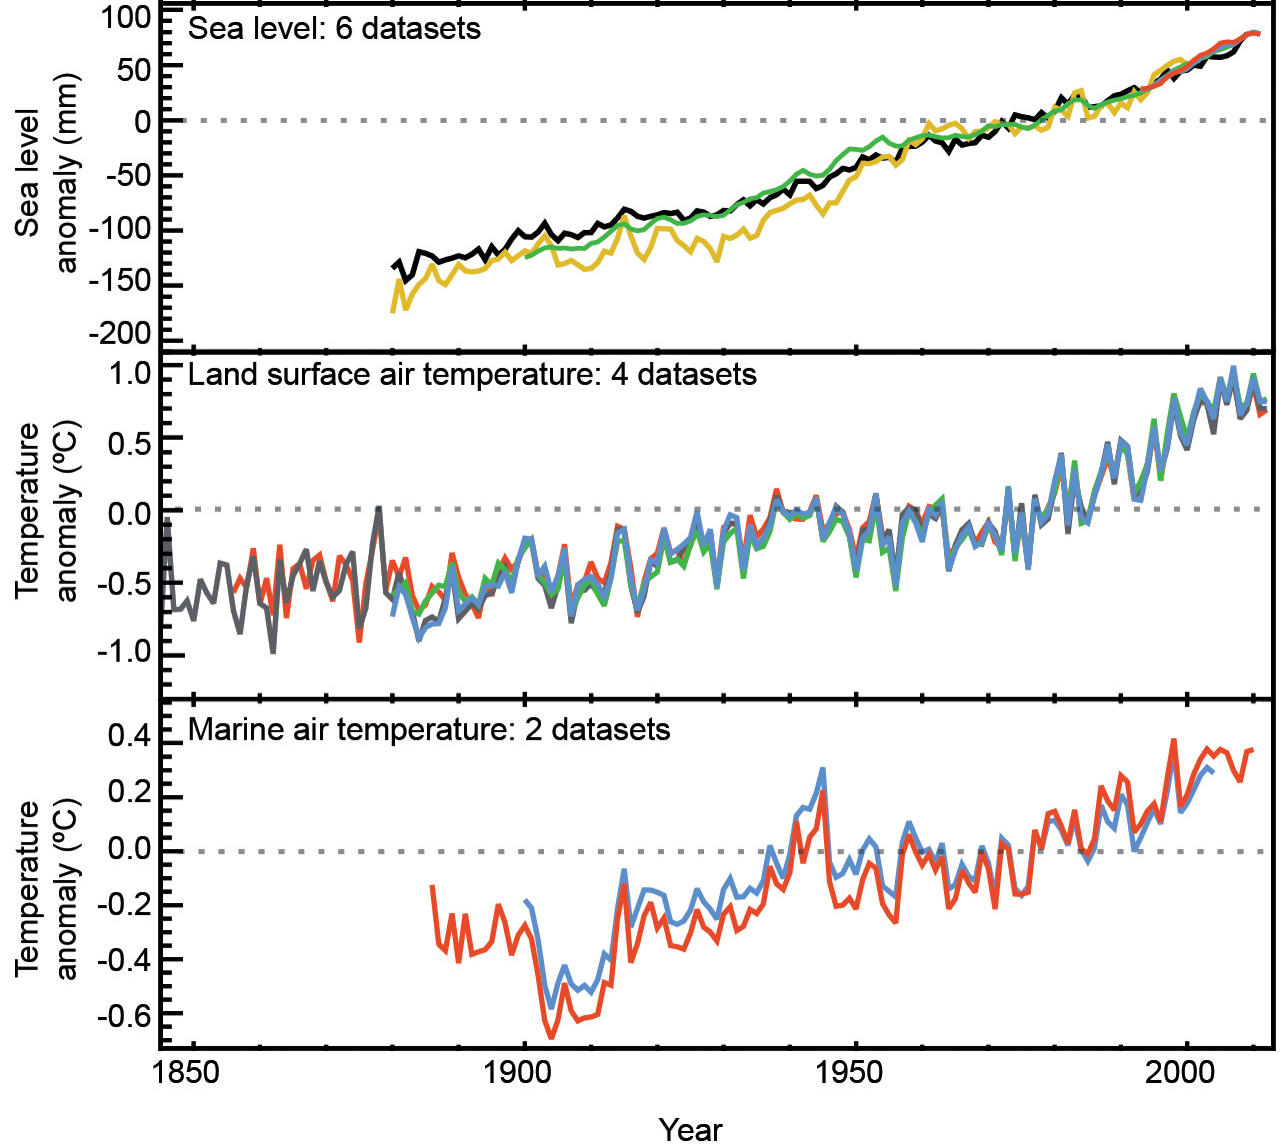
\includegraphics[width=\columnwidth]{../images/ipcc-ar5-wg1-temp-sea-level-collage.png}
            \caption{\href{http://www.ipcc.ch/report/ar5/syr/}{IPCC 2014}}
        \end{center}
        \end{figure}
    \end{columns}
    \end{adjustwidth}
\end{frame}

\begin{frame}
    \begin{adjustwidth}{-2em}{-1.5em}
    \vspace{-1mm}
    \begin{figure}
        \begin{center}
            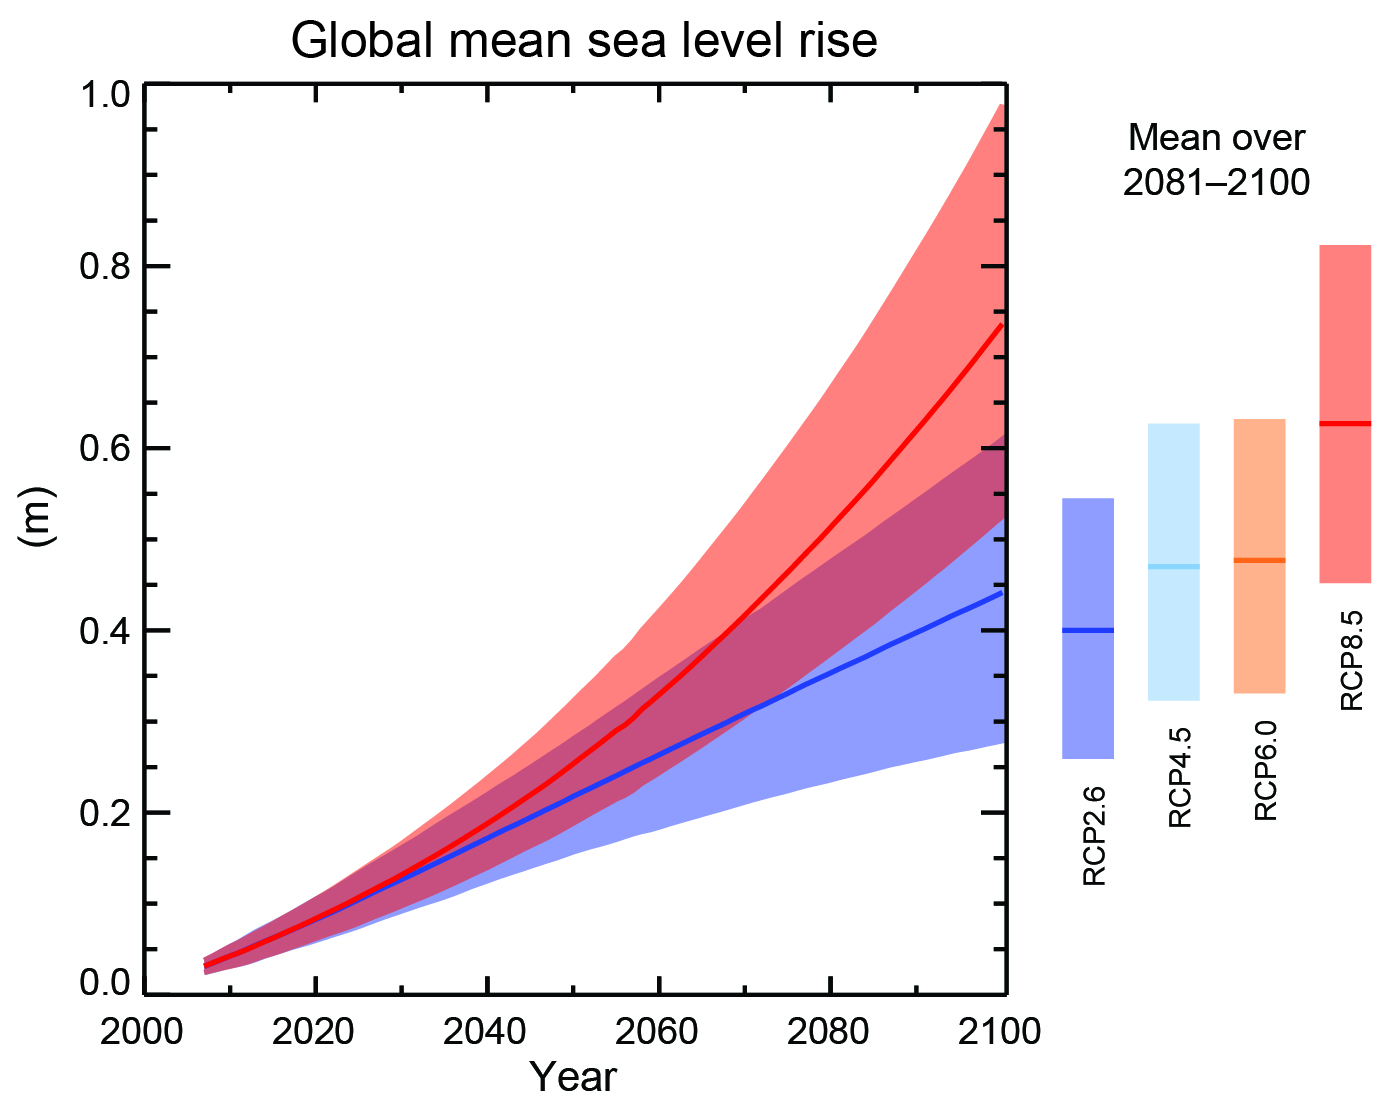
\includegraphics[width=0.8\textwidth]{../images/ipcc-ar5-wg1-sea-level-predictions.jpg}
            \caption{\href{http://www.ipcc.ch/report/ar5/syr/}{IPCC 2014}}
        \end{center}
    \end{figure}

    \vspace{-2mm}
    \uncover<2->{{\small
    Under the ``best-case scenario'' (RCP2.6), how much are sea levels
    predicted to rise by 2100 (relative to 1900)?  \wout{\tiny
        $0.2m+0.4\approx0.6m$}}}

    \end{adjustwidth}
    \note[item]{RCP = Representative Concentration Pathways}
\end{frame}

\begin{frame}[t]
    \begin{adjustwidth}{-2em}{-1.5em}
    \vspace{-3mm}
    Worst-case scenario (business as usual), how much will the average global
    temperature increase by 2100 (relative to 1900)? \wout{$1+4\approx5\dC$}

    \begin{figure}
        \begin{center}
            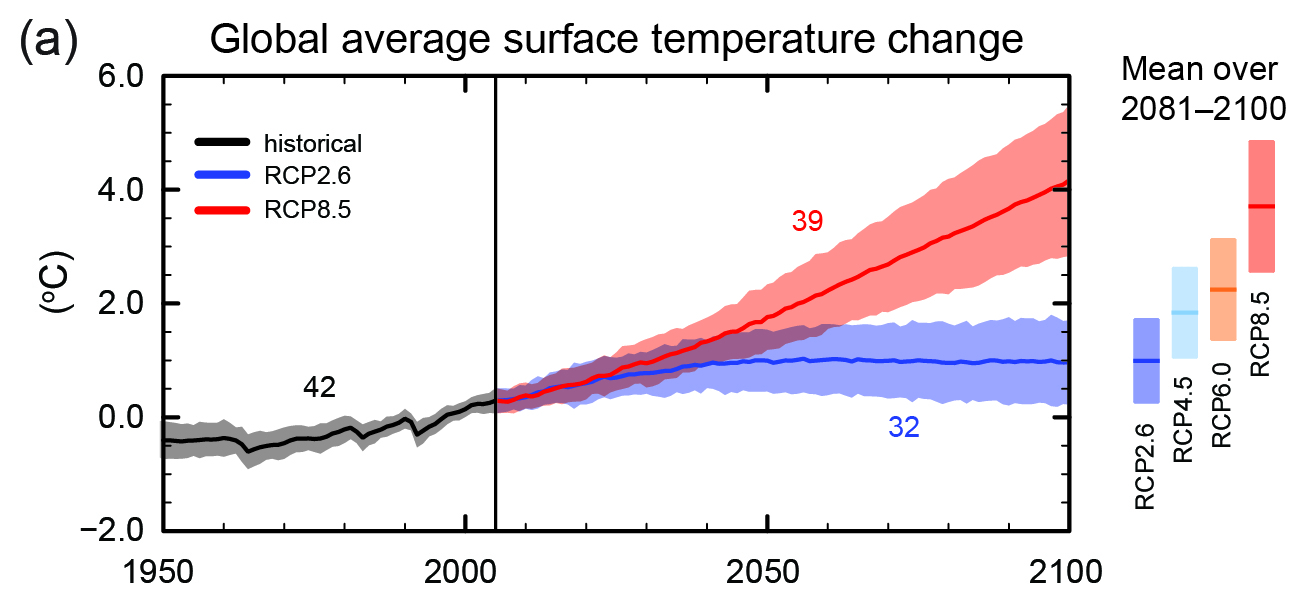
\includegraphics[width=1.0\linewidth]{../images/ipcc-ar5-wg1-temp-predictions.jpg}
            \caption{\href{http://www.ipcc.ch/report/ar5/syr/}{IPCC 2014}}
        \end{center}
    \end{figure}

    \vspace{-3mm}
    \uncover<2->{
        What does this mean for average land air temperature?
        
        \nbox{Average land air temperature will increase even more.}
    }
    \end{adjustwidth}
\end{frame}
    
\begin{frame}
    Get a worksheet from your TA. Please print your names legibly. \\

    \vspace{1cm}
    Work in teams of 3---middle person is the scribe (should do the writing).
    Make sure that you can explain your reasoning for each question. 
\end{frame}

\section{II. What are the consequences of global warming?}

% \begin{noheadline}
% \begin{frame}
%     \begin{columns}
%         \column{0.2\textwidth}
%             Interpret these graphs \\

%         \column{0.9\textwidth}
%         \vspace{-4mm}
%     \begin{figure}
%         \begin{center}
%             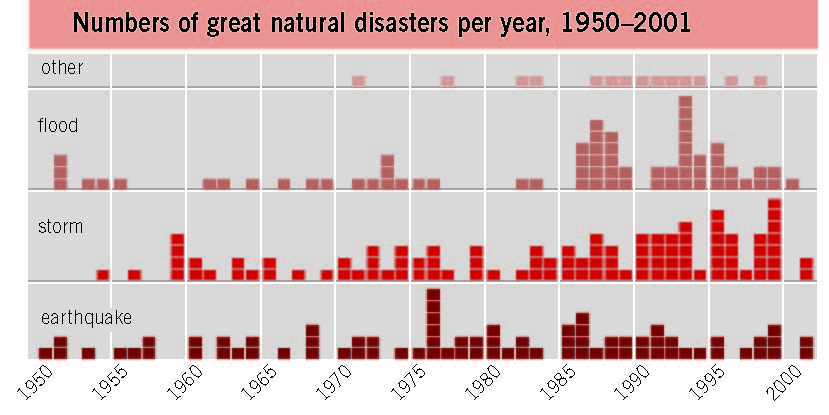
\includegraphics[width=0.8\textwidth]{../images/un-environment-programme-number-of-disasters.jpg}
%             \caption{\tiny UN Environment Programme}
%         \end{center}
%     \end{figure}

%     \vspace{-10mm}
%     \begin{figure}
%         \begin{center}
%             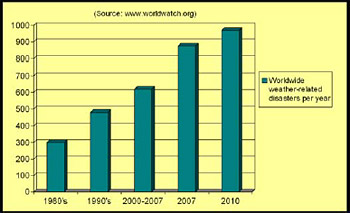
\includegraphics[width=0.75\textwidth]{../images/world-watch-institute-weather-disasters.jpg}
%             \caption{\tiny WorldWatch Institute}
%         \end{center}
%     \end{figure}
%     \end{columns}
% \end{frame}
% \end{noheadline}

\begin{frame}
    \vspace{-2mm}
    \begin{figure}
        \begin{center}
            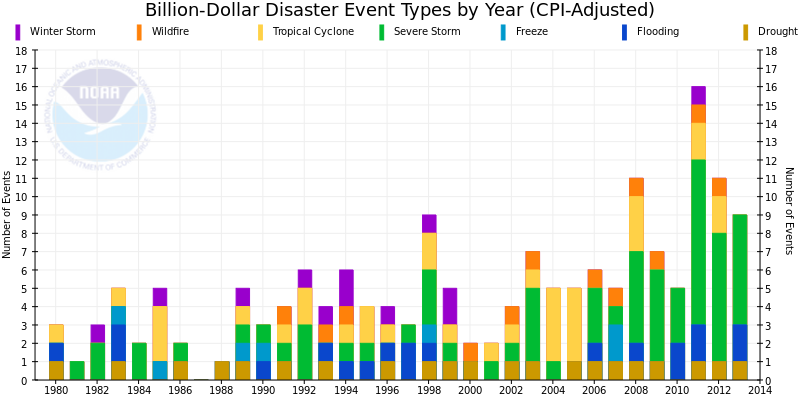
\includegraphics[width=0.65\textwidth]{../images/noaa-billion-dollar-disasters.png}
        \end{center}
    \end{figure}

    \vspace{-4mm}
    \begin{figure}
        \begin{center}
            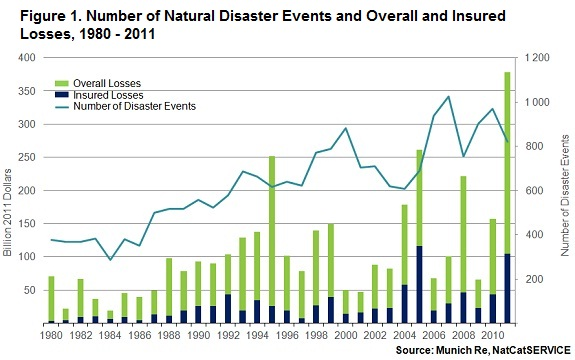
\includegraphics[width=0.65\textwidth]{../images/world-watch-institute-disaster-costs.jpg}
            \caption{\tiny WorldWatch Institute}
        \end{center}
    \end{figure}
\end{frame}


\section{III. What can we do to mitigate climate change?}

\clickerslide{
\begin{frame}
    \begin{clickerquestion}
        \item What are the pros and cons of planting trees as a way of
            reducing atmospheric CO\sub{2}?
 
        \begin{clickeroptions}
            \item Pros: dead trees absorb CO\sub{2};  Cons: living trees
                release CO\sub{2}.
            \item \clickeranswer{Pros: living trees absorb CO\sub{2} and are
                    long-lived; Cons: difficult to do at appropriate scale.}
            \item Pros: can be done anywhere; Cons: no established proof of
                efficacy.
            \item Pro: There is established evidence of efficacy; Con:
                Technologically difficult and expensive.
        \end{clickeroptions}
    \end{clickerquestion}
\end{frame}
}

\clickerslide{
\begin{frame}
    \begin{clickerquestion}
        \item After years of deliberations, USA and China have reached a
            long-term agreement to reduce CO\sub{2} emissions. In general, why
            are developing countries resisting such agreements?

        \begin{clickeroptions}
            \item \clickeranswer{Developed countries have much higher per
                    capita emission rates.}
            \item \clickeranswer{They want developed countries (the source of
                    most past emissions) to act first.}
            \item \clickeranswer{Emission reductions in developed countries is
                    largely due to the outsourcing of manufacturing to
                    developing countries.}
            \item \clickeranswer{They want to use ``cheap'' energy (fossil
                    fuels) to improve economic growth and quality of life.}
        \end{clickeroptions}
    \end{clickerquestion}
\end{frame}
}


\end{document}
